
%%%%%%%%%%%%%%%%%%%%%%% file typeinst.tex %%%%%%%%%%%%%%%%%%%%%%%%%
%
% This is the LaTeX source for the instructions to authors using
% the LaTeX document class 'llncs.cls' for contributions to
% the Lecture Notes in Computer Sciences series.
% http://www.springer.com/lncs       Springer Heidelberg 2006/05/04
%
% It may be used as a template for your own input - copy it
% to a new file with a new name and use it as the basis
% for your article.
%
% NB: the document class 'llncs' has its own and detailed documentation, see
% ftp://ftp.springer.de/data/pubftp/pub/tex/latex/llncs/latex2e/llncsdoc.pdf
%
%%%%%%%%%%%%%%%%%%%%%%%%%%%%%%%%%%%%%%%%%%%%%%%%%%%%%%%%%%%%%%%%%%%


\documentclass[runningheads,a4paper]{llncs}

\usepackage{amssymb}
\setcounter{tocdepth}{3}
\usepackage{graphicx}
\usepackage{lscape}
\usepackage{url}
\urldef{\mailsa}\path|{wendpanga-francis.ouedraogo,frederique.biennier}@liris.cnrs.fr|
\urldef{\mailsb}\path|{philippe.merle}@inria.fr|    
\newcommand{\keywords}[1]{\par\addvspace\baselineskip
\noindent\keywordname\enspace\ignorespaces#1}

\begin{document}

\mainmatter  % start of an individual contribution

% first the title is needed
\title{Contextualised security operation deployment through MDS@Runtime architecture}

% a short form should be given in case it is too long for the running head
\titlerunning{Lecture Notes in Computer Science: Authors' Instructions}

% the name(s) of the author(s) follow(s) next
%
% NB: Chinese authors should write their first names(s) in front of
% their surnames. This ensures that the names appear correctly in
% the running heads and the author index.
%
\author{Wendpanga Francis Ouedraogo%
\thanks{Please note that the LNCS Editorial assumes that all authors have used
the western naming convention, with given names preceding surnames.}%
\and Fr\'ed\'erique Biennier \and Philippe Merle}
%
\authorrunning{Gestion Contextualis\'ee de la S\'ecurit\'e}
% (feature abused for this document to repeat the title also on left hand pages)

% the affiliations are given next; don't give your e-mail address
% unless you accept that it will be published
\institute{Universit\'e de Lyon, CNRS INSA-Lyon, LIRIS UMR 5205, 20 avenue Albert Einstein, 69621 Villeurbanne Cedex, France\\
Inria Lille - Nord Europe, Parc Scientifique de la Haute Borne, 40 avenue Halley, 59650 Villeneuve d'Ascq, France\\
\mailsa\\
\mailsb\\}

%
% NB: a more complex sample for affiliations and the mapping to the
% corresponding authors can be found in the file "llncs.dem"
% (search for the string "\mainmatter" where a contribution starts).
% "llncs.dem" accompanies the document class "llncs.cls".
%

\toctitle{Lecture Notes in Computer Science}
\tocauthor{Authors' Instructions}
\maketitle

\begin{abstract}
The development of Collaborative Business leads to new challenges for corporate Information Systems (IS) operation such as interoperability, elastic deployment and security management in dynamic contexts. To fit the interoperability and elas-ticity challenges, Security Oriented Architecture and Cloud based organization are more and more used. The agility provided by the  middleware interconnecting the different IS components.
\keywords{MDS@Runtime, SecaaS, Business Process, Cloud Computing, SCA, FraSCAti}
\end{abstract}

\section{Introduction}
The development of Collaborative Business strategies leads to reorganize the corporate information system deployment in order to increase its agility. Taking advantage of the agility and interoperability of SOA, collaborative Business Process can efficiently be built by composing business services depending on business needs. Nevertheless, such collaborative organization challenges contextualized security deployment as a same business service may be used in different collaborative context and orchestrated using different runtime environment.
To fit this challenge, we've proposed to extend the Model Driven security approach to capture information and services protection requirements using an “end user oriented” set of questions to capture the patrimonial importance of these elements so that confidentiality, availability, integrity requirements can be consistently defined and used to annotate the Business Process specification. Then we use a model driven generation process to define the security policies associated to the services implementing the collaborative Business Process.
These security policies are seen as an abstract Model@Runtime protection specification. Depending on the runtime environment different security services must be selected and orchestrated to fulfill the protection requirements. To this end, we propose a SecurityModel@Runtime component that intercepts the service invocation, extracts its security policy and orchestrates the required protection services depending on the execution environment before launching the “functional” service. 
After presenting briefly the context and state of the art limits, we detail our SecurityModel@Runtime, paying attention on the way it can be plugged on the service execution middleware before showing the impact on the execution performances due to the policy interpretation.

\section{From MDS to MDS@Runtime}
The increased importance of Collaborative Business strategies leads to reorganize the corporate information system deployment in order to increase its agility and interoperability so that common Business Process supporting these collaborative organisation can be efficiently designed and deployed. Taking advantage of the agility and interoperability of SOA and Cloud environments, such collaborative Business Process can be built by composing business services before deploying them on cloud platforms depending on the needs. This leads to a "de-perimetrised" information system organization, as business services can be selected,  composed and orchestrated in various contexts, challenging a consistent and contextualised Business service protection.
For example (Fig~\ref{fig:bp}), setting a e-government service to improuve a scholarship management process
 lead to the development of a collaborative "on-line" e-governement organisation allowing both students, grant administration and academic partners to share students curriculum information. To this end, a common Business Process associated to scholarship business feature is built, combining services and personal workflows from both grant adaministration and academic partners, challenging new security features such as partner authentication, access control on the student information non repudiation...  

\begin{figure}  
\centering
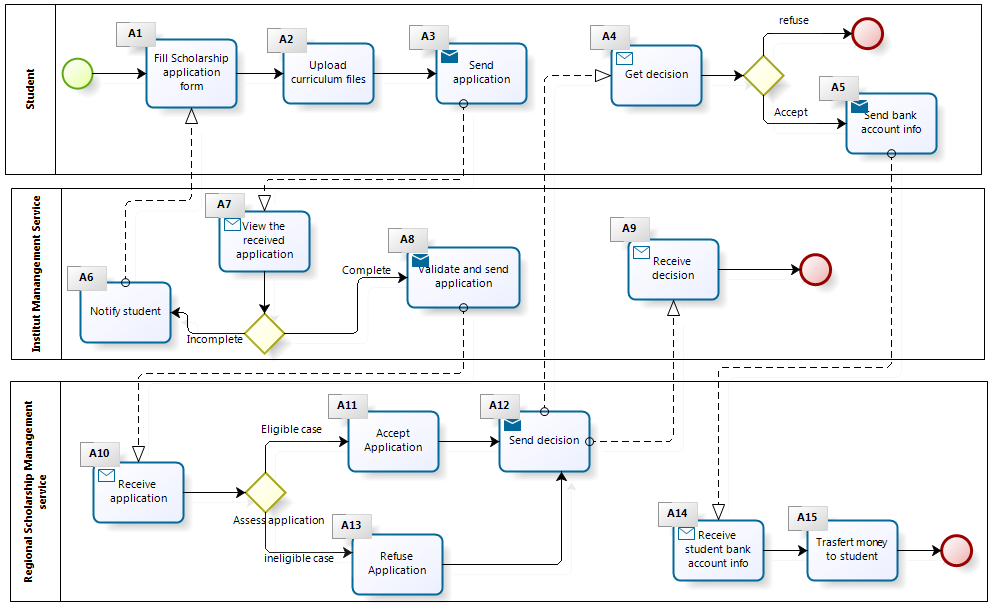
\includegraphics[height=200pt, width=320pt]{BRPE_Eng.png}
\caption{Scholarship management process}
\label{fig:bp}
\end{figure}

\subsection{Securing services}
Depending on the perceived security risks / system vulnerabilities, different security requirements can be set. Based on the ISO/IEC 27002, the OASIS Service Reference Model (~\cite{OAS06}) defines different security requirements (Condidentiality and privacy management, Integrity, Authentication, Authorisation, Availability and Non Repudiation) that  requires the deployment of security means from the network layer (which is rather focused on the availability requirement and protection against deny of service attacks)and transport layer (which has to provide secured confidential channel between tranmitters and receivers) to the Application layer which manages most of the security requirements (Authentication, Authorisation, Non repudiation, confidentiality and privacy...). Different standards such as WS-Security, SAML, XACML, BSLA...(see XX FIG ou tableau XX) have been developped to support these security requirements implementation.
Such protection means can either be deployed directlty in the service operation or "attached" to the service interface specification. To this end, Security policies can be used to specify the required protection levels and means to be deployed, allowing an easier "upgrading" of protection requirement. 
For example, authenticating students and or academic partners, building secured communication channels and establishing non repudiation features could be achieved by combining different protection means (see the secvurity policy that could be attached to the service) (Fig~\ref{fig:policy}). By this way, service operations are not affected while security requirements are taken into account.

\begin{figure}  
\centering
\includegraphics[height=135pt, width=380pt]{scholarshipPolicies.png}
\caption{Security policies associated to « Scholarship » resource.}
\label{fig:policy}
\end{figure}


\subsection{MDS for Services}

Different methods can be used to set a consistent security policy, based on vulnerability and threats models as EBIOS, MEHARI, OCTAVE, SNA... However, they are complex and designed for a perimetrised environment and are not "end-user" oriented. To overcome these limits, business architects should be able to define security policies while building new business process. To this end, Model Driven Security can be used to attach security requirements specification in the Business Process and generate adapted security policies. In previous work, we have proposed in ~\cite{OBG12} to enrich the MDS approach with a security pattern engineering strategy to capture protection requirements and deployment platform information to generate automatically the security policies that will be attached to the different services (see Fig~\ref{fig:mds}).
In our example,the student curriculum activity and the related information must be protected in the new "openned" context. This confidentiality requirement impacts both application layer which will be in charge of the access control (i.e. authentication and authorisation management) and the transport layer (Fig~\ref{fig:policy}). 
To provide a consistent protection of the information system, the security policies must be used to compose and orchestrate security services accordingly. Taking into account more precise information on the execution context could improve both the service operation performance and the protection level, avoiding under / over protection deployment. In our example, each employee of the academic partners can accede to the curriculum activity from the already secured partner network. Once the security policy is attached to the collaborative workflow, access control including a systematic authentication is required to fulfill the non repudiation requirement as well as log features and network encryption, despite the secured access provided by the corporate infrastructure (namely authentication to unlock the workstation and secured infrastructure). (Table ~\ref{tab:tab1}) shows a comparison of service execution time with / without authentication and authorization.
\begin{table}
\caption{Execution time comparaison (ms)}
\begin{tabular}{|l|l| }
\hline
Business Service without access control & Business Service with access control \\
  \hline
 59 ms & 72 ms\\
    \hline
\end{tabular}
\label{tab:tab1}
\end{table}

To avoid this costly over-protection or risky under-protection depending on the runtime environment vulnerability, we propose to turn these security policies as Model@runtime so that they can be analysed to select, compose and orchestgrate the most convenient security services depending on the exact runtime environement. This requires a new architecture to "outsource" the security management as a new high-level service that can be plugged on the execution middleware. In the next section, we'll present this new architecture and a proof of concept based on the Frascati middleware.







\begin{figure}  
\centering
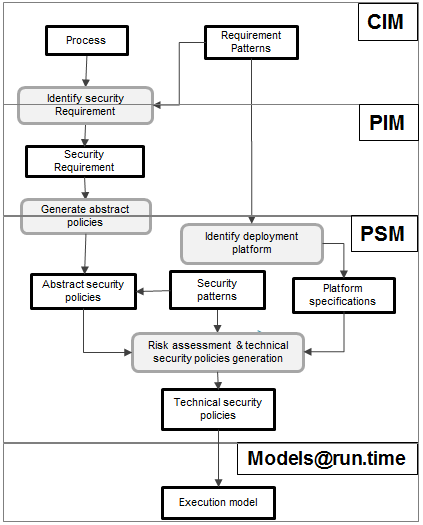
\includegraphics[height=200pt, width=160pt]{mds.png}
\caption{Security policy generation process based on MDS}
\label{fig:mds}
\end{figure}




\subsection{MDS@Runtime: Adapting security deployment in service operation}
Probl\`eme pos\'e : le d\'eploiement dynamique de la s\'ecurit\'e pour \'eviter l’over / under protection. Dans un contexte dynamique, on ne peut plus consid\'erer qu’on va mettre toute la s\'ecurit\'e dans le code du service / invoquer les politiques  une fois pour toute car il faudrait alors faire toutes les invocations en syst\'ematique et l’over protection est particuli\`erement couteuse. Ici On pourrait mettre un exemple de mesure du service qui invoque les services d’authentification /autorisation et monter le diff\'erentiel en temps d’ex\'ecution. Ce constat conduit donc \`a renoncer \`a la vision « compil\'ee » de la s\'ecurit\'e, c’est-\`a-dire \`a faire une pr\'e-orchestration des diff\'erents services de s\'ecurit\'e mais \`a adopter une vision « interpr\'et\'ee » de la s\'ecurit\'e pour reporter les derni\`ere phases de g\'en\'eration sous forme d’une s\'election / composition / orchestration de services de s\'ecurit\'e au moment de l’ex\'ecution.
Deuxi\`eme axe : il faut expliquer que la solution doit pouvoir \^etre adapt\'ee  diff\'erents contexte donc il faut repenser l’architecture traditionnelle pour int\'egrer cette \'etape de s\'ecurisation dynamique. On termine donc avec le sch\'ema d’architecture mis dans le ppt de Philippe et son explication : on sur une architecture existante et on construit  un intercepteur plugg\'e sur le middleware. Cet intercepteur permet de r\'ecup\'erer les invocations de service puis invoque un m\'ediateur de s\'ecurit\'e charg\'e d’interpr\'eter les politiques. A partir de ce parsing on int\`egre le mod\`ele de plateforme pour d\'ecider si on doit ou pas composer un chaîne de services de s\'ecurit\'e (qui peuvent \^etre soient des services de s\'ecurit\'e propre au SI ou une offre de services de s\'ecurit\'e g\'en\'erique qu’on peut mettre en SecaaS). Puis on « orchestre » localement l’invocation de ces services avant d’invoquer le service fonctionnel
On ajoute un diagramme de composants pour expliquer le d\'etail de l’architecture.

Implementing a Service Oriented Architecture (SOA) requires a middleware for both integration and distributed communication. Middleware plays an intermediary role between the client and the service provider. It is a software component which is located between the operating system and business applications and offers an abstraction high level for building distributed applications. It allows business services integration and management, and provides access to various external services ~\cite{SHLP05}. It is an integration solution which implements a fully distributed architecture (deployment on multiple nodes), providing services such as data processing or routing based on the content (CBR), and a higher level of interoperability by use systematically standards such as XML, Web Services specifications and WS-* ~\cite{Lou08}.
 
 Fig~\ref{fig:archi} shows our architecture organization. 
\begin{figure}[ht]  
\centering
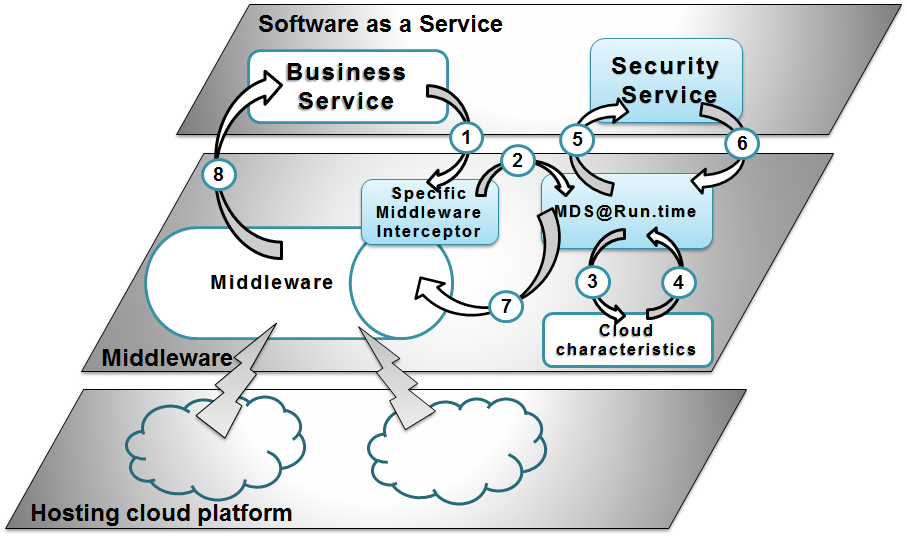
\includegraphics[height=180pt, width=280pt]{architecture1.PNG}
\caption{\textbf{Plugin security components on FraSCAti}}
\label{fig:archi}
\end{figure}


\section{Implementation : MDS@Runtime with FraSCAti}
\subsection{Frascati Organisation}
Expliquer ce qui est n\'ecessaire de savoir sur FraSCAti pour comprendre la suite du papier

FraSCAti ~\footnote{\url{http://frascati.ow2.org}}~\cite{SMF09}~\cite{SMR12} is a middleware based on the OASIS Service Component Architecture (SCA) standard to build service-oriented and adaptable business applications. FraSCAti applications can be deployed in different clouds (Amazon EC2 , Amazon Elastic BeanTalk , Google App Engine, CloudBees , etc.)~\cite{MRS11}~\cite{PHM12}. The adaptability at the design is based on the fact FraSCAti platform was designed as a plugin-based architecture to adapt to different execution environments and to select on demand, the required application functionality to compose its platform. The adaptation to the execution is based on FraSCAti reflective features, which mean the capacity for applications introspection and reconfiguration at runtime. This middleware allow getting more agile and reconfigurable SI. However, this poses obvious security problems.
\subsection{Composite SecaaS}

The \textbf{Security as a Service} composite includes various security services which allow protecting resources and business services according to security "as a service" approach. This composite contains the following components (see Fig.~\ref{fig:SecaaS}):
\begin{figure}[ht]  
\centering
\includegraphics[height=190pt, width=230pt]{Secaas1.PNG}
\caption{\textbf{Security as a Service} composite.}
\label{fig:SecaaS}
\end{figure}

\begin{itemize}
\settowidth{\leftmargin}{{\Large$\square$}}\advance\leftmargin\labelsep
\itemsep8pt\relax
\renewcommand\labelitemi{{\lower1.5pt\hbox{\Large$\square$}}}

\item The \emph{SecaaS} component is the composite entry point. It receives from \emph{Mediator} component, the security policies to be applied. It is responsible for analyzing these policies, to identify the type of security services (authentication, authorization , etc. . ) to call.
\item The \emph{Authentication} component is used to prove the user identity  ( of human or other service). This component receives from SecaaS component, the policy rule to apply, extract information about the security pattern and invokes the security mechanism to be applied. It can be a weak authentication mechanism such as login / password or Strong Authentication such as One Time Password (OTP) or two factors authentication. This authentication component includes subcomponents such as \emph{SSORegistry} ( SSO Single Sign On) component used to store information about sessions authentication  and allow to retrieve user information without restarting authentication.

\item The \emph{Authorization} component allows managing access to resource or service and allows grant or deny the user access to the service. As the authentication , it receives the security policy rule and invokes the authorization mecanism to be applied. This mecanism can be  based on a authorization by role (RBAC) implemented by XACML authorization protocol or a simple Access Control List ( ACL).
\item The Encryption component provides data and messages encryption and decryption mechanism. It also provides secure protocols using  to secure communication (SSL).
\item The \emph{Integrity} component ensures the data and messages integrity exchanged by using messages signature or hash functions.
\item The \emph{Nonrepudiation} component is responsible for recording user actions (authentication, access to data or service, data modification / destruction, etc . ). This information can then be used for auditing and monitoring.
\item The \emph{Availability} component is responsible for the services availability providing access to the service or a clone (redundant service) thereof if the original target service is unavailable. This component also provides backup mechanism to restore system data and services after disaster.


\end{itemize}

The Encryption, Integrity and nonRepudiation components can use security protocols such as WS-Security XML Encryption and XML Signature which provide encryption and signing  exchanged messages mechanisms.



\subsection{Composite MDS@Runtime}



FraSCAti provides a framework for programming, deploy and execute components achieving as services which are OASIS SCA standard compliant. To ensure the business processes security deployed on cloud infrastructures, we pro- pose a security framework based on SCA components which can be plugged to FraSCAti platform. The framework includes two composites, which are components that contain sub-components. The composite MDS@Runtime intercepts calls of business services and invoke security services which implement security policies. This composite include five main components (see Fig~\ref{fig:mdsAtRuntime}):

\begin{figure}[ht]  
\centering
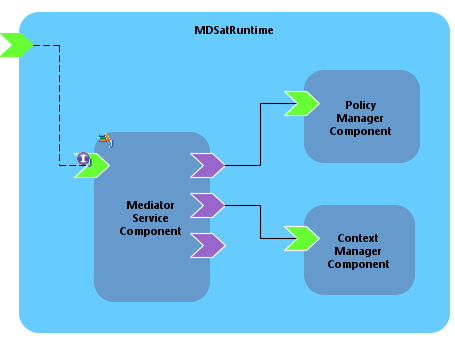
\includegraphics[height=120pt, width=200pt]{mdsAtRuntimeComponent1.png}
\caption{\textbf{MDS@Runtime} composite.}
\label{fig:mdsAtRuntime}
\end{figure}

\begin{itemize}
\settowidth{\leftmargin}{{\Large$\square$}}\advance\leftmargin\labelsep
\itemsep8pt\relax
\renewcommand\labelitemi{{\lower1.5pt\hbox{\Large$\square$}}}

\item The \emph{Mediator} component is responsible for analyzing called service requests intercepted by the  \emph{Intent} component and  encapsulated by the \emph{Request} component. It also identify the security policies rules associated to business service with which the client needs to interact. Thus, through the \emph{Request} component, the \emph{Mediator} receives information of the services involved in the interaction. This information is used to get policies associated to resources (the business services functionality implemented by service operation). These policies are then analyzed and orchestrated by the \emph{Mediator} to call the required security services.
\item The \emph{PolicyManager} component manages the policies. It receives from the \emph{Mediator} the resource or service reference requested and the policy file link. It returns to the \emph{Mediator} the list of policies to apply.
\item The \emph{ContextManager} component analyses security policies associated to services and identifies the different policies to be applied according to the user context, the execution environment and security policies associated to the client and service provider. It also provides to the \emph{Mediator} component information such as policies and policies rules related to the execution context. These policy rules are used by the \emph{Mediator} component to call the technical security services.
\end{itemize}


\subsection{FraSCAti Intent for MDS@Runtime}
\begin{itemize}
\settowidth{\leftmargin}{{\Large$\square$}}\advance\leftmargin\labelsep
\itemsep8pt\relax
\renewcommand\labelitemi{{\lower1.5pt\hbox{\Large$\square$}}}
\item The \emph{Intent} component is responsible for detecting and intercepting business services invoked  by clients. This component uses the aspect-oriented programming (AOP) techniques implemented in FraSCAti to perform actions before, during and after each business services invocation. These techniques use the Apache CXF interception mechanisms embedded in FraSCAti. Once clients purpose are captured ( eg Apache CXF messages generated by a service call), they are then formatted to be interpreted by the \emph{Mediator} component to ensure safety.
\item The \emph{Request} component plays the intermediary role between FraSCAti middleware and security services. It provides a bidirectional interface that allows the component Intent to formalize the interaction messages received from the FraSCAti platform and also to specify orders toward the FraSCAti platform which performs some technical actions. This component ensures a total independence between the FraSCAti middleware and our security system, allowing one hand, the security services,  to be able to deploy and run on any other middleware and second hand, to deploy on a specific platform just the required security services.
\end{itemize}
\begin{figure}[ht]  
\centering
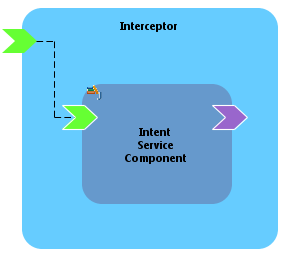
\includegraphics[height=120pt, width=140pt]{interceptorComponent1.png}
\caption{\textbf{Interceptor} composite.}
\label{fig:mdsAtRuntime}
\end{figure}

\section{Evaluation}

\label{sec:exemple}
Pr\'esentation du use-case (reprendre de SAR) et expliquer les 2 contextes de fonctionnement du SI bourse : travaille uniquement \`a la r\'egion ou ouverture dan la logique de egov. Cela impose donc de connecter les I et surtout de modifier la partie « operation » pour permettre d’int\'egrer des services d’authentification / autorisation. On se focalise sur un service d’acc\`es au dossier de bourse pourg\'erer l’\'evaluation.
On peut mettre \'eventuellement une comparaison des temps avec une invocation syst\'ematique de l’authentification puis authentification / autorisation d’acc\`es pour montrer l’int\'er\^et de notre approche (sauf si on le met dans le point 2). On termine avec l’\'evaluation des temps de r\'eponses en montrant que l’intent et le d\'eploiement du m\'ediateur restent acceptables par rapport au cas de d\'eploiement syst\'ematique des services de s\'ecurit\'e.


To illustrate our approach, we propose to use a process of the scholarship award by the region, which collaborate with the institut in a e-government logique. In this example, each student fill a scholarship application form, upload various documents (resume, cover letter, diplomas, ...) and submit its request. Then, the institute manager, view and check each student application data to ensure that it is compliant before sends it to the region. At the regional level, applications are analyzed by agents, who decide to award or not scholarships based on eligibility criteria. Once the decision is taken by these agents, a notification is sent to each student and each school principal is informed about the decision. Students whose applications have been accepted are then requested to send their bank account information to the region in order to trasfert scholarship money.
In this esxemple, the student application contains personnal data which require to be protected. For that, we have to secure these data against the unauthorized access.  
We propose to focus on the student data activity 
we propose a simple use case to control access to the student data. During our approach based MDS patterns implementation, security policies are automatically generated (see Fig.~\ref{fig:policy}) and associated to "Scholarship" service (see Fig.~\ref{fig:wsdl}).



 
 
These policies specify that the service has an operation named "ViewStudentData", which is considered as a resource (line 2 in Fig.~\ref{fig:policy}). This resource requires authentication (lines 2-8) by login /password (line 4) with the reference to the user authentication checking file specified on line 5. Besides authentication, access control (lines 9-16) using ACL (line 12), with time constraints (line 10) should be applied to this resource. Fig.~\ref{fig:acl} describes the contents of the  autorization file. It shows that users can access the resource at specific hours (between 6am and 12pm for user "user1").
 
 
\begin{figure}
\centering
\includegraphics[height=55pt, width=380pt]{scholarshipAcl.png}
\caption{Authorization file « AccessControlList.xml ».}
\label{fig:acl}
\end{figure}


These security policies, which are in fact our security model at runtime, are associated with the service description (see Fig.~\ref{fig:wsdl}), including the reference to the policy file (line 3). This allows during business service execution to identify the security policies to be applied.
\begin{figure}  
\centering
\includegraphics[height=120pt, width=380pt]{scholarshipWSDL.png}
\caption{Link policy file with operation \emph{«ViewStudentData»} of the \emph{«Scholarship»} service WSDL.}
\label{fig:wsdl}
\end{figure}

\begin{figure}  
\center
\includegraphics[height=105pt,width=380pt]{scholarshipComposite.png}
\caption{Link \emph{Scholarship} component with \textbf{MDS@Runtime} component.}
\label{fig:gestionEtudiant}
\end{figure}


In order to enforce these security policies, the "Scholarship"  Web Service binding (line 6 Fig. ~\ref{fig:gestionEtudiant}) requires to be associated to the \textbf{MDS@Runtime}\footnote{The XML \emph{requires} attribute is the mean for FraSCAti to weave an aspect on SCA component.} composite. This specification allows to intercept calls of the service and invoke the  MDS@Runtime composite before invoking the business service itself.
\begin{figure} 
\center
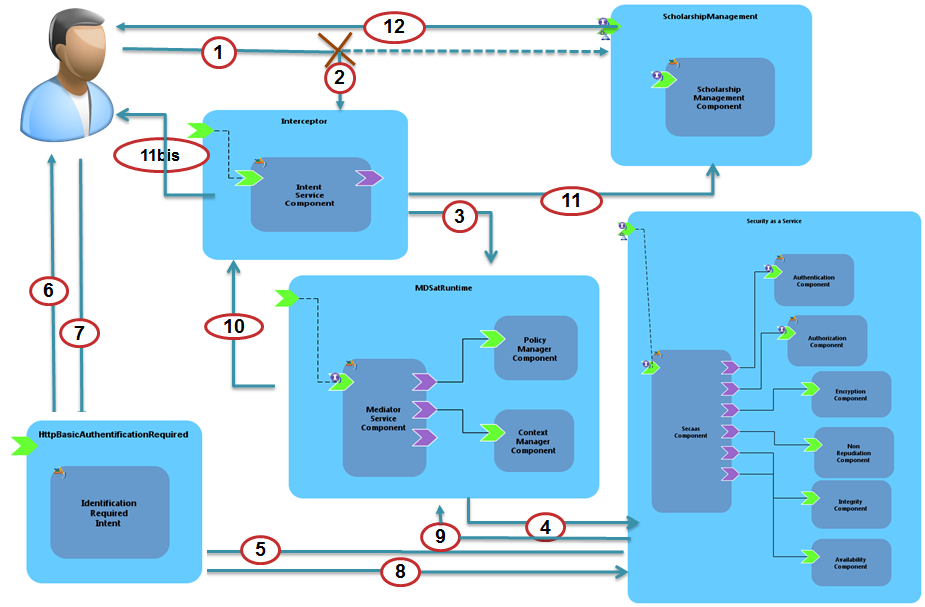
\includegraphics[height=200pt, width=320pt]{process.png}
\caption{\emph{«Scholarship»} service execution process including   \textbf{MDS@Runtime} execution.}
\label{fig:process}
\end{figure}


Fig. ~\ref{fig:process} shows the complete execution process. The " Scholarship " Service  calling by the user (1) is intercepted by the \textbf{MDS@Runtime} \emph{Intent} component (2) which format the intercepted Apache CXF message to initialize\emph{Request} component. The \emph{Intent} component invokes the \emph{Mediator} component that retrieves from the component \emph{Request}, information on the service(service name and operation invoked and the  the service WSDL description). Then the \emph{Mediator} parse the service description in order to retrieve the security policy. Security policy reference is sent to \emph{PolicyManager} component which return to the \emph{Mediator} the list of security policies to apply. The \emph{Mediator} then orchestrate policies and calls \emph{SecaaS} component which applies security policies ( 3). For this, the SecaaS component analyse  policy , identifies the corresponding security service then invokes it. In our example it is the authentication by login/password service which is first invoked. If the user is not logged yet, it will be redirected to an identity service provider (4) ( the \emph{HttpBasicAuthentification} service) to collect user identity (5) and (6). This identity is then returned (7) to authentication service which check the user identity. If the test is positive, an authentication token is generated. The token contains a unique identifier which ensures user has been authenticated. It also allows to find the real identity of the user and to automatically re-authenticate as SSO during user access to other services . The checking result is then returned to the \emph{Mediator} (8) which continues policies orchestration until policies performed return success before invoking the business service. In our example, after authentication , the authorization service will be invoked. If  ( authorization ) successful, access is granted to business service and business service is finally invoked ( 9) (10 ), otherwise an error message is returned to the user (9a) .
\begin{figure}  
\center
\includegraphics[height=150pt,width=390pt]{seqGestionEtudiant0.png}
\caption{Interactions inside  \textbf{MDS@Runtime} composite.}
\label{fig:sequence}
\end{figure}


Thank to FraSCAti Explorer tool ~\cite{SMF09}, it is possible, as shown in Fig. ~\ref{fig:sequence}, to follow the invocation of  \textbf{MDS@Runtime} composite components as a UML sequence diagram.


\begin{table}

\caption{Components execution times}
\begin{tabular}{@{}*{3}{|p{3.1cm}}|@{} }
\hline
Component & Run time execution(ms)   & Rate of run time \\[0.2cm]
  \hline
  FraSCAti \& CXF \& Business service & 59&  76\%\\
 FraSCAti Interceptor & 2&  3\%\\ 
 MDS@Runtime & 4&  5\%\\
 Authentication& 10& 13\%\\
 Autorization & 3& 4\%\\
 \hline
   Total & 78& 100\%\\
    \hline

\end{tabular}
\end{table}


\begin{figure}[ht]  
\centering
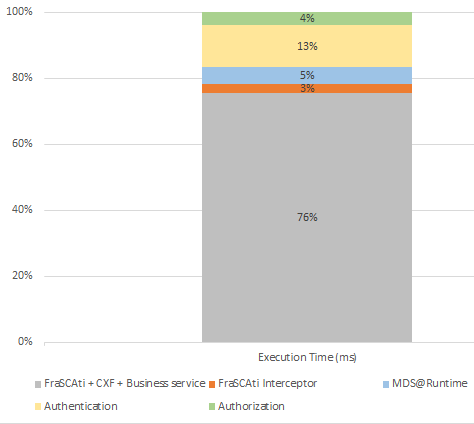
\includegraphics[height=220pt, width=250pt]{runtimeAssessment1.PNG}
\caption{\textbf{Runtime assessment according to the involved components
}}
\label{fig:SecaaS}
\end{figure}








\section{Related works}

Il faut repartir de la partie SOTA de SAR traduite et compl\'eter avec les travaux sur MDS. Il faut aussi restructurer le tableau comparatiftableau comparatif



Security is IS non-functional property which take an important place in the robust systems development. It have to be taken into account in the early step of software development. So, security models must be added at the design step with a high level of abstraction in order to be managed by the business architects before being transformed to allow services suitable protection at the deployment.
Several studies have proposed to integrate security during the information system design time as UMLSec and SecureUML which extend UML to security specifications. In UMLSec, security requirements are described using stereotypes and tags security (integrity, confidentiality ...). ”Constraints” using a formal semantics based on UML models are associated to the UMLSec model and are used to assess security requirements and identify potential vulnerabilities. Unlike UMLSec, SecureUML focuses on the management of access rights. It is a meta-model based on RBAC model and defines an abstract syntax to annotate UML diagrams with access control information. However, these both solutions provide a descriptive view of protection needs and do not allow to generate security mechanisms conforming to these specifications. To overcome this limit, suggested, based on UMLSec, an model-driven security ( MDS- Model Driven Security) approach providing engineering and retro engineering security approach tank to set of tools. Model Driven Security (or MDS )  ~\cite{LS09} ~\cite{LZN14} is an approach that describes the security requirements modeling process at a high abstraction level by adapting the MDA ( Model Driven Architecture) approach to the field of security  ~\cite{BDL03}~\cite{CSB08} using security models based on UML or security annotations which are more specifically for business processes ~\cite{SSL09}~\cite{WMS09}. MDS enables the system security requirements modeling and the security policy generation during the design step. It also allow dynamic policy updates and monitoring at runtime. To do this, information associated to the system ( provided by stakeholders) are expressed in a Domain-Specific Language (DSL) before being automatically transformed into technical security rules, avoiding as far as possible human intervention. Due to these advantages, several studies have focused on the use of the MDS approach to secure business process and led to frameworks definition like OpenPMF, SECTET and BPSec. These frameworks (see Table 1) are based on UML models and security annotations to define security requirements, and transform them automatically to security policies. However, these frameworks don’t provide means to identify process security requirement: they assume that the specification was made beforehand. Whereas, to secure a process, a business analyst should first identify the security constraints to meet and the security level to provide for each process activity, service and data before considering to define the specifications. This security constraints identification step is overshadowed by these framework, restricting their use to the security experts which can be a braking force to the rapid deployment of collaborative applications built by services compositions. Moreover, in addition to their unsuitability for end users, these frameworks do not allow to adjust the service protection level based on the deployment and execution environment. This can be an additional threat in the case of under-protection (some vulnerabilities can be forgot) or a loss of efficiency in the case of overprotection (security means being unnecessarily deployed). This is particularly for deployment in a cloud computing environment. Indeed, according to the type of cloud (public, private...) and the service level (XaaS) provided by the cloud provider, the platform protection level have to be adjusted. The using of MDS approach by these framework should take into account platforms context to adapt the security to the deployment environment.


\begin{landscape}
\begin{table}

\caption{Comparaison of frameworks based on MDS}
\begin{tabular}{@{}*{6}{|p{3.1cm}}|@{} }
\hline\noalign{\smallskip}
Framework & Our solution   & Open PMF & SECTET & BPSec & []\\[0.2cm]
  \hline
  Modeling approach & EMF+ATL+ transformation Ad-hoc  & UML+DSL interne & UML2 + SECTET DSL & UML +QVT & Ad hoc\\
  Abstraction level & CIM- PIM- PSM-code  &  PIM- PSM-code  &  PIM- PSM-code &  CIM- PIM (UML Use case )&  PIM- PSM\\
  End user oriented & Yes & No & No & Yes & No\\
  Policy auto-generation & Yes & Yes & Yes & x & YES\\
  Infrastructure dependent & Yes & No & No & No & No\\
  Execution context dependent & Yes & No & No & No & No\\
  Security criteria &  Authentication, Autorization,  Integrity, Encryption, Non repudiation, Availability, Privacy & Authentication, Autorization,Monitoring & Encryption, Non repudiation, Authentication & Non  r\'epudiation, 
Privacy,  intrusion Detection,  Access control, Autorization & Autorization \\
  Policy monitoring & No & Yes & No & No & No\\
  Policy auto-update & No & Yes & No & No & No\\
  SecaaS & Yes & No & Yes & No & No\\
  Security standards  & XACML,  SAML,  WS-Security & XACML  & SAML,  WS-policy, XACML & x & XACML\\

\hline
\end{tabular}
\end{table}
\end{landscape}






\section{Conclusion}
Ouvrir sur la vision de bout en bout et agragation de politique par exemple
\label{sec:end}
La s\'ecurisation de processus m\'etiers d\'eploy\'es dans les nuages passe par la prise en compte du contexte m\'etier du processus mais aussi du contexte de d\'eploiement et d’ex\'ecution. Afin d’assurer la protection des services du processus, nous proposons d’\'etendre l'approche MDS jusqu’\`a	 la phase d’ex\'ecution afin de s\'electionner \`a	 l’ex\'ecution uniquement les politiques de s\'ecurit\'e qui doivent s’appliquer au contexte. Notre architecture de s\'ecurit\'e, conçue comme un service pluggable sur l'intergiciel FraSCAti, intercepte \`a	 la vol\'ee les interactions du client avec les services et orchestre les services de s\'ecurit\'e correspondants aux besoins sp\'ecifi\'es dans les politiques de s\'ecurit\'e en fonction du contexte de d\'eploiement. Notre impl\'ementation avec FraSCAti permet d’utiliser notre service de s\'ecurisation pour un d\'eploiement de processus collaboratifs dans un environnement multi-nuages. L'agr\'egation des politiques de s\'ecurit\'e et l'optimisation des invocations aux services de s\'ecurit\'e (\'eviter les invocations doublons) constituent les prochaines extensions de notre service de gestion de la s\'ecurit\'e \`a	 l’ex\'ecution (MDS@Runtime).





\begin{thebibliography}{4}

\bibitem{BDL03} D. Basin, J. Doser, and T. Lodderstedt. Model Driven Security for Process
Oriented Systems. In 8th ACM Symposium on Access Control Models and
Technologies (SACMAT 03), pages 100–109. ACM, 2003.
\bibitem{CSB08}M. Clavel, V. Silva, C. Braga, and M. Egea. Model-Driven Security in Practice : An Industrial Experience. In 4th European Conference on Model Driven
Architecture : Foundations and Applications (CMDA-FA 08), pages 326–337,
2008.
\bibitem{Lou08} A. Louis. Bus de Service ESB, Nouvelle technologie pour l’int\'egration. Livre
blanc, Petals Link, 2008.
\bibitem{LS09} U. Lang and R. Schreiner. Model Driven Security Management : Making
Security Management Manageable in Complex Distributed Systems. In Workshop on Modeling Security (MODSEC08) - International Conference on Model
Driven Engineering Languages and Systems (MODELS), 2009.
\bibitem{MRS11} P. Merle, R. Rouvoy, and L. Seinturier. A Reflective Platform for Highly Adaptive Multi-Cloud Systems. In International Workshop
on Adaptive and Reflective Middleware (ARM’11) - 12th ACM/IFIP/USENIX
International Middleware Conference, pages 14–21. ACM, 2011.
\bibitem{OBG12} W. F. Ouedraogo, F. Biennier, and P. Ghodous.
Adaptive Security Policy Model to Deploy Business Process in Cloud Infrastructure. In 2nd International Conference on Cloud Computing and Services Science (CLOSER 2012), pages 287–290, 2012.
\bibitem{PHM12} Fawaz Paraiso, Nicolas Haderer, Philippe Merle, Romain Rouvoy, and Lionel
Seinturier. A Federated Multi-Cloud PaaS Infrastructure. In 5th International
Conference on Cloud Computing (CLOUD’12), pages 392–399. IEEE, 2012.
\bibitem{SHLP05} M.-T. Schmidt, B. Hutchison, P. Lambros, and R. Phippen. The Enterprise
Service Bus : Making Service Oriented Architecture Real. IBM Systems Journal, 44 :781–797, 2005.
\bibitem{SMF09}Lionel Seinturier, Philippe Merle, Damien Fournier, Nicolas Dolet, Valerio
Schiavoni, and Jean-Bernard Stefani. Reconfigurable SCA applications with
the FraSCAti Platform. In IEEE International Conference on Services Computing (SCC’09), pages 268–275. IEEE, 2009.
\bibitem{SMR12}L. Seinturier, P. Merle, R. Rouvoy, D. Romero, V. Schiavoni, and J.B. Stefani. A component-based middleware platform for reconfigurable service-oriented architectures. Software : Practice and Experience, 42(5) :559–583, 2012.

\bibitem{SSL09}A. R. Souza, B. L. Silva, F. A. Lins, J. C. Damasceno, N. S. Rosa, P. R. Maciel,
R. W. Medeiros, B. Stephenson, H. R. Motahari-Nezhad, J. Li, and C. Northfleet. Sec-MoSC Tooling - Incorporating Security Requirements into Service Composition. In 7th International Joint Conference on Service-Oriented Computing (ICSOC-ServiceWave 09), pages 649–650, 2009.

\bibitem{WMS09}C. Wolter, M. Menzel, A. Schaad, P. Miseldine, and C. Meinel. Model-driven business process security requirement specification. Journal of Systems Architecture (JSA), pages 211–223, 2009.

\bibitem{LZN14} Levi Lucio, Qin Zhang, Phu Hong Nguyen, Moussa Amrani, Jacques Klein, Hans Vangheluwe, Yves Le Traon: Advances in Model-Driven Security. Advances in Computers 93: 103-152 (2014)

\bibitem{OAS06}Organization for the Advancement of Structured Information Standards (OASIS): “Reference Model for Service Oriented Architecture 1.0: OASIS Standard”, 12 October 2006.
\end{thebibliography}

\end{document}